
\documentclass[acmtog]{acmart}

\usepackage{graphicx}
\usepackage{subcaption}
\usepackage{hyperref}

\graphicspath{ {./images/} }

\AtBeginDocument{%
	\providecommand\BibTeX{{%
			\normalfont B\kern-0.5em{\scshape i\kern-0.25em b}\kern-0.8em\TeX}}}

\setcopyright{acmcopyright}
\copyrightyear{2023}
\acmYear{2023}
\acmDOI{XXXXXXX.XXXXXXX}

\begin{document}
	\title{Land Use Classification Project Results}
	
	\author{Thai La}
	\email{vtl932@usask.ca}
	\orcid{1234-5678-9012}
	\affiliation{%
		\institution{University of Saskatchewan}
		\streetaddress{105 Administration Pl}
		\city{Saskatoon}
		\state{Saskatchewan}
		\country{Canada}
		\postcode{S7N 5A2}
	}
	
	\keywords{Satellite, Image, Classification, LandUse, GeoSpatial}
	
	\maketitle
	
	\section{Introduction}
	This report detail the results, the hyperparameter study for tuning, and road blocks that were encountered during this project..\\ \\
	\href{https://git.cs.usask.ca/vtl932/cmpt318_course_project}{The project repository can be found here}.\\
	\href{https://www.kaggle.com/datasets/apollo2506/eurosat-dataset?select=EuroSAT}{The Kaggle Dataset can be found here}.
	
	\section{Results}
	The approach I took for this problem is to use a convolution neural network to learn good features for the images and then classified the images based on the learned features using a fully connected neural network.
	\\
	I used transfer learning for my convolutional layers. The architecture I used for the convolution neural network was the VGG16 architecture. I only kept the convolutional layers and disposed of the dense layers that came along with the VGG16 architecture; this allowed me to adapt the pre-learned model to work on my data set because the images of my data set were of size 64 x 64. I froze the convolutional layers so that its weights were no longer trainable, then I added 2 final layers for the neural network, then were:
	
	\begin{itemize}
		\item Flatten: to flatten the output of the convolutional neural networks and input it into the dense layer.
		\item Dense: this dense layer is the output layer and contained only 10 units.
	\end{itemize}
	The activation function for the Dense layer was a softmax activation function.
	I used an epoch of 6, batch size of 16, a learning rate of 0.001, the Adam optimizer, the sparse categorical cross entropy loss, and the accuracy metric.
	\\
	I was able to achieve an accuracy of 87\% for the test set. Please reference the figures in the next page for the accuracy and loss graph, and the confusion matrix.
	
	\section{Hyperparameter study}
	I performed a hyperparameter study on the trained model. A total of 5 sweeps were performed, each sweep with different hyperparameters.
	\begin{itemize}
		\item Sweep 1: Epochs: 10, Learning Rate: 0.001, Batch Size: 16
		\item Sweep 2: Epochs: 10, Learning Rate: 0.001, Batch Size: 32
		\item Sweep 3: Epochs: 8, Learning Rate: 0.0001, Batch Size: 64
		\item Sweep 4: Epochs: 5, Learning Rate: 0.00001, Batch Size: 128
		\item Sweep 5: Epochs: 15, Learning Rate: 0.001, Batch Size: 128
	\end{itemize}
	From figure 3a and figure 3b, you can see that sweep 1 consistently performs the best, thus I used the hyperparameters of sweep 1 for the model. However, instead of 10 epochs, I had only trained the model for 6 epochs, since any further training will result in overfitting.
	
	\section{Road-blocks}
	All the road blocks I ran into were implementation-based as it was my first time using tensorflow.\\
	One roadblock was when I tuned the hyperparameters of my model, such as epochs, batch size, etc., it did not correctly fit the model again since the weights were persistent. To resolve this, I re-compiled the model every time I changed the hyperparameters.
	\\
	Another road block I ran into was how to convert the numpy-representation of the image into tensor-representation of the image so that I can make use of hardware acceleration provided by Tensorflow. To resolve this, I created a utility function that converted a numpy array into a tensor.
	
	
	
	\begin{figure*}[h]
		\centering
		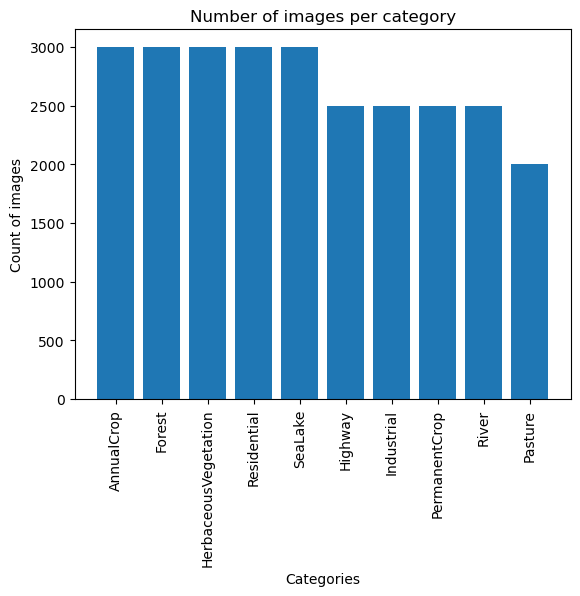
\includegraphics[scale=0.5]{../src/images/FinalResults/Final_Dataset_figure.png}\\
		Figure 1. Final Dataset Figure
	\end{figure*}
	
	\begin{figure*}[h]
		\centering
		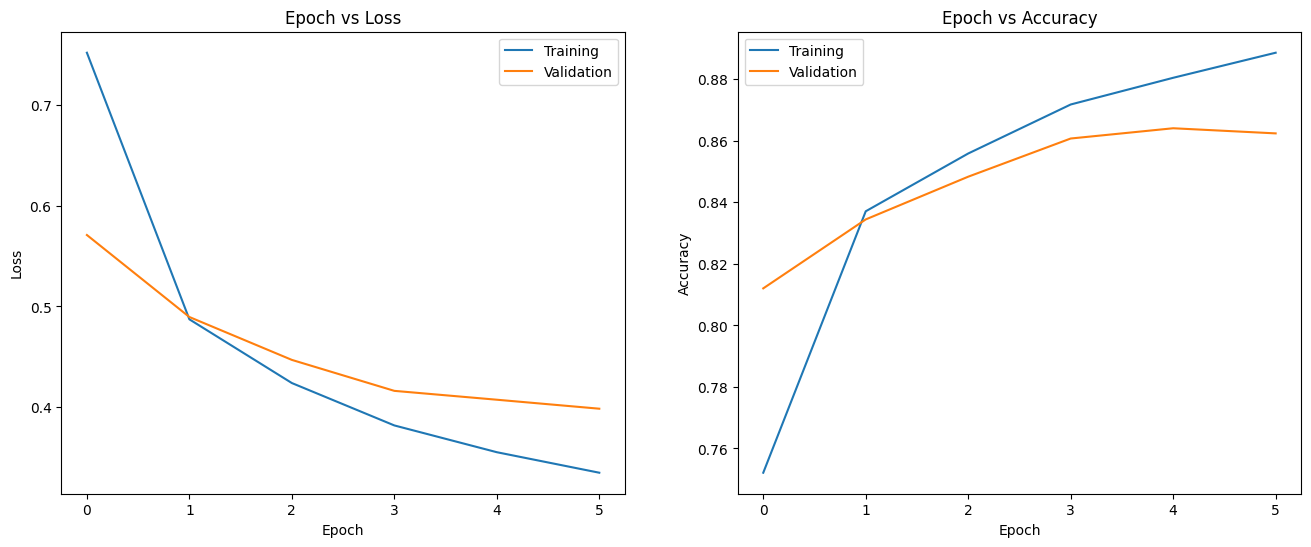
\includegraphics[scale=0.5]{../src/images/FinalResults/Final_Results_figure_a.png}\\
		Figure 2a. Final Results Figure (a) - Training and Validation Loss and Accuracy per epoch
		
		\vspace{2cm}
		
		\centering
		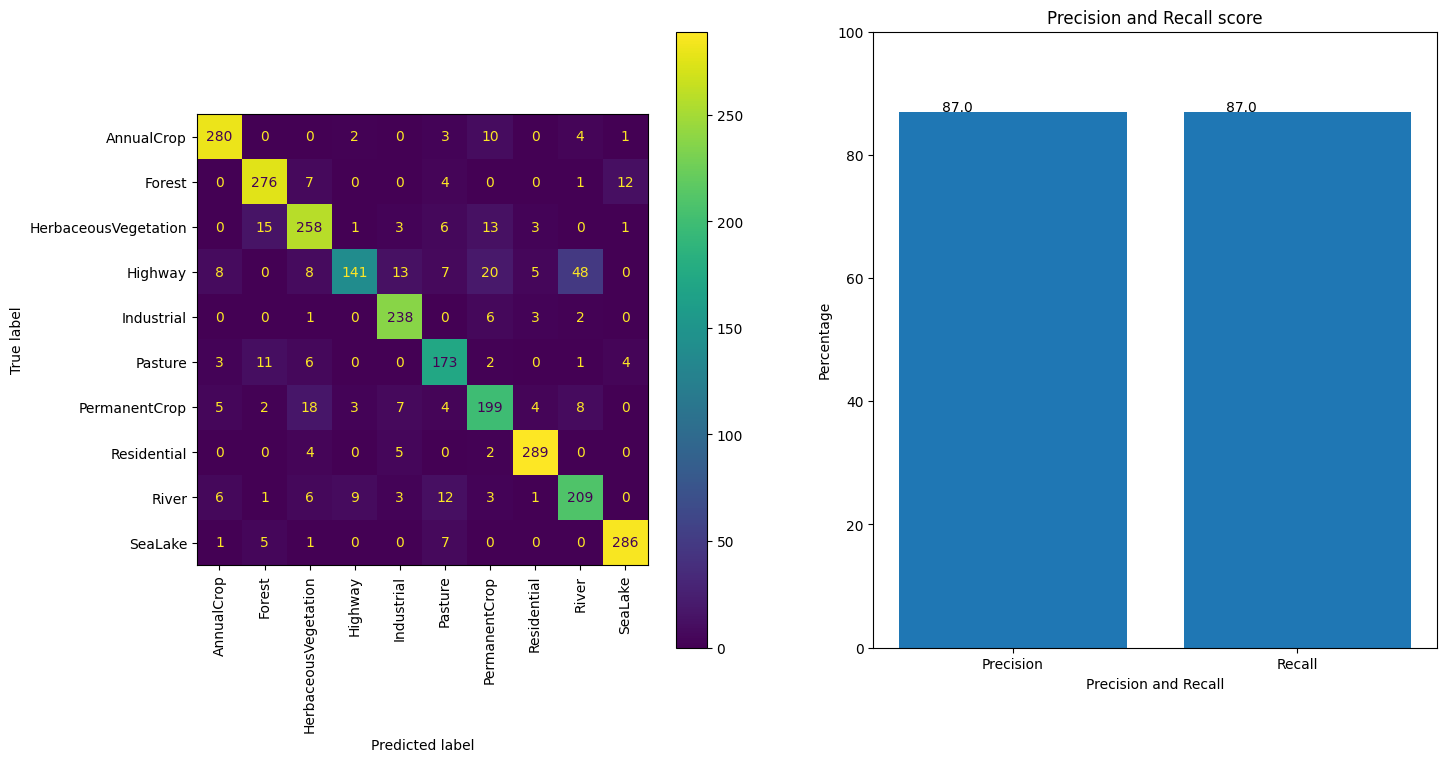
\includegraphics[scale=0.5]{../src/images/FinalResults/Final_Results_figure_b.png}\\
		Figure 2b. Final Results Figure (b) - Confusion matrix, precision and recall of prediction on the test set
	\end{figure*}
	
	\begin{figure*}[h]
		\centering
		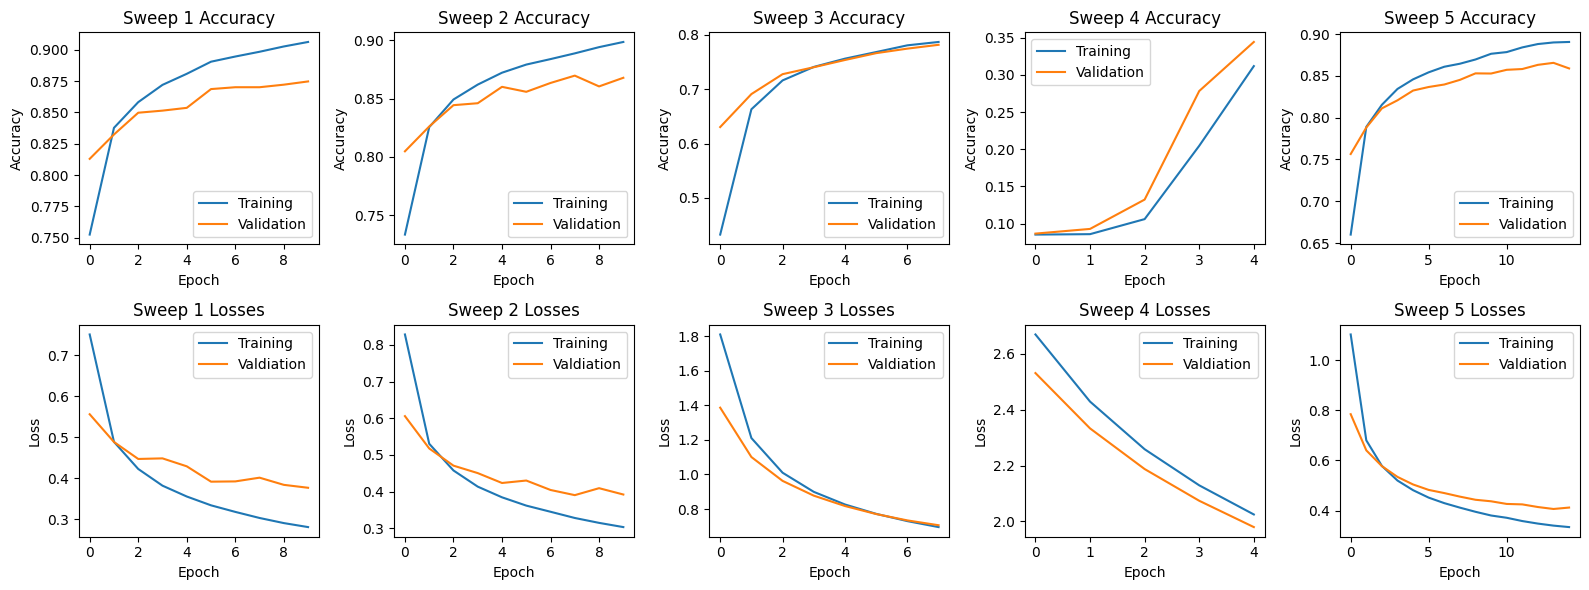
\includegraphics[scale=0.4]{../src/images/FinalResults/Additional_Results_figure_a.png}\\
		Figure 3a. Additional Results Figure (a) - Accuracy and Loss graphs per sweep
		
		\vspace{2cm}
		
		\centering
		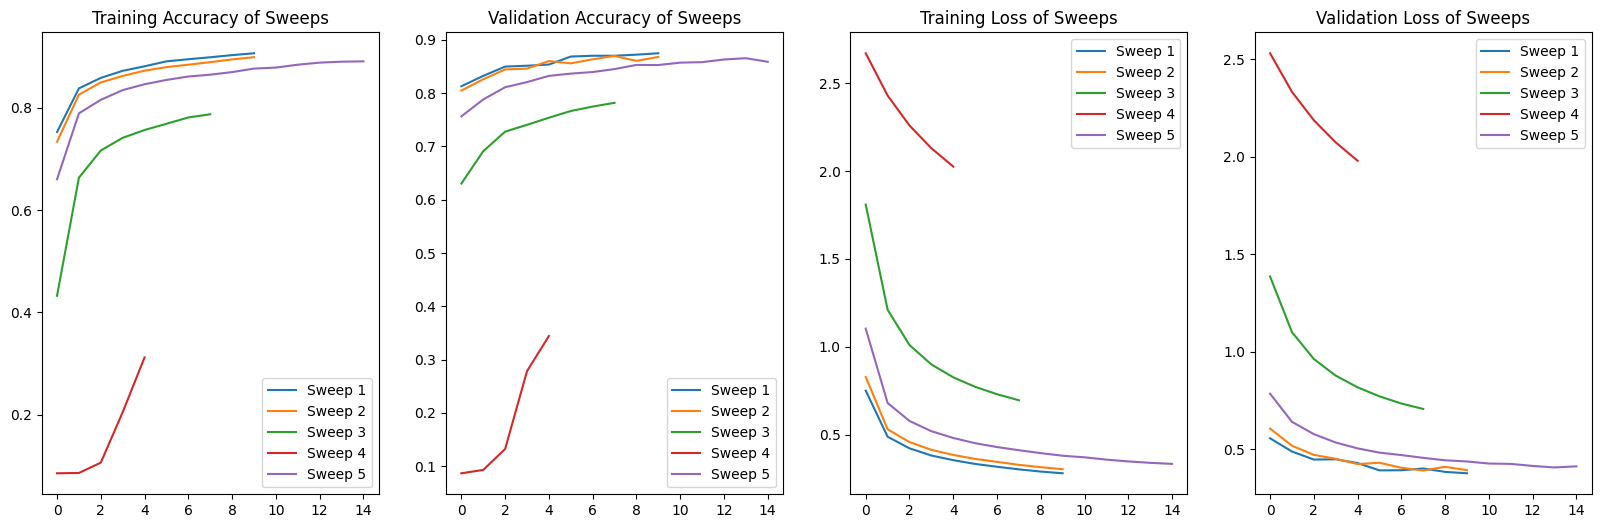
\includegraphics[scale=0.4]{../src/images/FinalResults/Additional_Results_figure_b.png}\\
		Figure 3b. Additional Results Figure (b) - Accuracy and Loss graph, aggregated sweeps
		
	\end{figure*}
	
\end{document}
\endinput
